\chapter{自然语言理解:从语言到逻辑}{From Language to Logic}
\label{chap:comprehension}

本章阐述如何对第\ref{chap:intro}章中的提到的假设1展开研究。根据该假设,我们认为, 借助于依存关系语法和传统逻辑与谓词逻辑的合理结合,将自然语言表达式转换成满足下列两个条件的逻辑表达方式是完全可行的:
\begin{itemize}
\item 包含该自然语言表达式的主要语义
\item 具体化自然语言表达式中存在的任何无法在语言到逻辑的转换消除的歧义,使得这些歧义能通过基于语境知识的逻辑推理后很直截了当地得到消除。
\end{itemize}

基于这样的假设,我们采用的自然语言方法是,首先利用链语法分析工具Link Parser[XXX],然后在此基础上搭建了一个用于依存关系抽取的工具RelEx,最后开发了一个新的逻辑关系抽取工具RelEx2Logic,通过超图的同态映射方式将句法结构转换成语义表示。该方法概念上的本质并不依赖这些特定的工具,而是具体的实现方法。

确切地说,如何将“自然语言理解系统”分解成不同模块以及如何进行不同模块之间的转换,取决于对语言学理论的选择。在2008-2012年期间,OpenCog中的自然语言理解模块采用如下流程:

文本 —> 分词/断句 —> 基于链语法的句法分析(Link Parser) —> 依存关系抽取(RelEx)—> 基于FrameNet的语义关系抽取(RelEx2Frame) —> 语义节点和关系链 (SemanticNodes \& Links)

2012年的时候我们对系统进行了一些简化,取消了对FrameNet的依赖,采用了如下的目前正在使用的系统:

文本 —> 分词/断句 —> 基于链语法的句法分析(Link Parser) —> 依存关系抽取(RelEx)—> 抽象的逻辑关系抽取(RelEx2Logic —> 语义节点和关系链 (SemanticNodes \& Links)

需要注意的是,目前的很多自然语言理解系统都有“词性标注”阶段,在我们目前使用的方法中,词性标注被绑定在句法分析阶段,对于Link Parser来说,词性已被作为单词的一个属性定义在词典里。尽管如此,如果能在Link Parser里使用先进词性标注技术,无疑能减少不少字典编写方面的工作,也能在一定程度上指导句法分析过程,因此也是有一定存在意义的。

本文的工作已经表明,上述系统中的各模块操作都是可行的,只需针对每一步制定相应的规则,或者通过有监督的机器学习方法来学习相应的规则,来指导其中的操作。针对本文自然语言理解方面的以下几个额外事项将在未来的研究中被实现:
\begin{itemize}
\item 使得各个子流程中所使用的规则,能很自然地支持基于持续经验增长的修正和泛化。
\item 使得语义理解能根据特定的语境来指导规则的选择。
\item 知道何时该打破规则,而根据语义的直觉指导相关操作。
\end{itemize}

另外需要注意的一点是,当使用基于规则的方法时,在规则的设计需要特别注意规则的可扩展性和可普及性,因为随着系统的经验增长,原先设计的规则可能无法被满足。

本章接下来的章节会系统介绍我们使用的自然语言理解系统中的各个子系统的工作原理和方法。

\section{链语法}{Link Grammar}

本小节主要介绍链语法的基本原理和方法,并分析了和语言形式主义的不同,同时指出其中的问题以及我们对其进行的一些改进。

链语法(Link Grammar)在1991年由 Daniel Sleator和Davy Temperley共同提出[XXX]。它和被广泛应用的依存语法类似,但两者也有很大的不同,比如链语法中两个单词的连接是无序的,而依存语法中有依存和被依存关系。链语法允许句子中的链接有环状结构,而依存语法是不允许环的存在的。链语法更倾向于语法理伦的词汇主义。

链语法的核心是链语法词典(Link Dictionary),词典中的每一个词都记录着一些特点的链接要求,这些链接要求通过一系列具有特定逻辑排序的链接子(connector)组合成的公式(Formula)收录在词典的相应词条里,链接子包含名称和后缀(“+”或“-”),后缀表示该链接子的指向方向,“+”表示该链接子指向右,“-”表示该链接子。如果两个词需要合法连接,则要求两个词首先有相同名称的链接子,且左边单词的链接子的连接方向必须指向右,右边单词的链接子的连接方向必须指向左。

链语法分析器(Link Parser)是基于链语法的句法分析器。使用链语法分析句子的时候,句法分析器对句子中的每个单词去查询链语法词典得到每个单词的链接要求,根据这些链接要求进行相应的链运算,便得到句子的链语法结构。 链语法判断句子是否合法,除了需要满足句子所有单词的链要求外,还要满足以下四个原则:

\begin{itemize}
\item 平面性(Planarity),链之间不能互相交叉。
\item 连通性(Connectivity),句子中的每个单词都必须有链和其他至少一个单词相连,形成连通图。
\item 顺序性(Ordering),公式中较左边的链接子必须和距离单词较近的单词链接,反之,公式中较右边的链接子必须和距离单词较远的单词链接。
\item 排它性(Exclusion),一对单词之间同时不能有两条链链接。
\end{itemize}

下面我们借用Sleator和Temperley的“Parsing with a Link Grammar”[XXX]中使用的例句来解释链语法分析的操作过程。
The cat chased a snake.
链语法分析器对上面的例子分析后产生如下结果:
 
由于我们对该链语法分析器做了不少的改进,所有我们这里给出的分析结果和Sleator和Temperley的原文中的结果以及发布在网上的分析器得到的结果会有细微的不同 ,后面章节会介绍我们做的改进 。

链语法认为在句子最前面加上一个虚拟词(通常用LEFT-WALL表示)是很有必要的,这样首先能保证链语法的“连通性“原则,使得句子最后的标点符号能与LEFT-WALL连接而不被孤立。另外,在本文的4.1.2节也提到,通过这样的虚拟词来追溯句子的头(主动词)也是非常方便可行的。上面的句法分析结果中出现的”RIGHT-WALL”是可选的,可以用于特殊标点符号的处理,但通常情况下只是用RW链与句子最后的标点符号相连。

前面提到链语法词典是链语法的核心,它包含所有常用的英文单词的链接要求。下方的表格列出上述例句中出现的单词以及它们在链语法词典里被定义的链接要求。
\begin{verbatim}
words	formula
a the	D+
snake cat	D- & (O- or S+)
chased	S- & O+
\end{verbatim}
如前面所述,链接要求限制了这些连接子必须按照一定的原则来分配,例如“the”只有一个向右的连接子D+,那么它只能和带有D-的单词形成合法的链接。而“snake”和“cat”都能和它相连,但根据链语法的“顺序性原则”,“cat”比“snake”近,所以“the”“cat”之间可以画一条D链,同样的道理,“chased”和“snake”之间可以画一条O链,以此类推。最终我们可以得到如下的结构图。需要注意的是,我们这里只是对链语法的工作原理做简单地介绍,因此忽略了链接子类型的子类型等细节,比如“cat”含有Ss+,“chased”含有链接子Ss-,,所以该句法结构图和我们上面列出的目前链语法分析器在连接类型上有点小出入。 

链语法分析器在对句子进行句法分析时,对句子中的每个单词,都会考虑下面两种变量:
\begin{itemize}
\item 该单词在链语法词典中对应的链接要求,即上面中的公式(Formula)
\item 该单词为了满足句子结构的一致性(Agreement)必须具备的特征属性
\end{itemize}

比如在上述例句中,对于单词“snake”,通过查询链语法词典,我们得到相应的公式“D- \& (O- or S+)”,同时该单词还有相应的特征属性如“时态(tense)”“人称(person)”等。但对于单词“the”,就不需要与一致性相关的变量。

链语法分析器中也使用简单的转换生成类似短语结构语法的句法分析结果,如下:
\begin{verbatim}
    (S (NP The cat)
           (VP chased
                (NP a snake ))
    .)
\end{verbatim}
在我们的工作中,对该短语结构用的不多,所以这里不做详细说明。我们会在下一节简单讨论链语法和短语结构语法的潜在关系。

\subsection{链语法与短语结构语法}{Link Grammar vs. Phrase Structure Grammar}

讨论各种语法的优缺点不是本文的重点,本节只将链语法和典型的短语结构语法做个简单的对比来讨论它们的潜在联系。一般来说,依存语法和短语句法也有相应的联系[参见图XX],但不同的依存语法使用不同依存关系集合,也有不同的属性,分析起来会比较复杂,也不是本文的研究内容,所以我们这里不做详细阐述。
图XX:依存句法分析和短语句法分析对比
A comparison of dependency (above) and phrase-structure (below) parses.
In general, one can be converted to the other (algorithmically); dependency
grammars tend to be easier understand.
图片来自[XXX]

简单起见,这里只列出两条有用的观察结果,基于这些观察结果,我们不难发现,在链语法中也隐形存在短语结构。这是有一定道理的,但由于自然语言的复杂性,某些情况下可能也不是那么简单。
\begin{itemize}
\item 链语法中的公式是符合语法范畴的。例如,前面提到的例句中“chased”的链结构是“S- \& O+”,在范畴语法中,这意味着,“chased”属于这样的语法范畴,该范畴中的词都满足链结构“S- \& O+”。换句话说,链语法中每一个“公式”都对应依附该公式的单词的范畴。 
\item 词之间的链接也可以看成是短语的核心词(head)之间的链接。例如,在例句“The cat chased a snake”中,“chased”和“snake”之间有链接O,那么也可以说,以“chased”为核心词的短语和以“snake”为核心词的短语之间有链接O。换句话说,可以理解成,链语法为了简化,通过核心词来识别短语。
\end{itemize}

\subsection{识别句子的中心词}{Identifying the Head of a Sentence}
链语法从词的局部着手关注任意两个词之间的关系,在一定程度上忽略了语言的层次结构。因此标准的链语法也存一些弊端,有不少语言现象会被链语法拒绝认为是不合法的结构。比如并列结构、介词短语等。在本文的研究过程,我们对链语法做了很多的改进,由于链语法的链接要求非常复杂,修改链语法词典可能牵扯到很多语言学上的问题。但这不是本文的研究重点,所以这里不一一列出我们做过的改进,只简单的列出几项较大的改进:
\begin{itemize}
\item 改进了链语法对连词的处理
\item 改进了链语法对量词的处理
\item 识别句子的中心词。
\end{itemize}

链语法分析器(Link Parser)是一个开源工具,包括链语法词典,我们所有的改进都发布在 http://abisource.com/projects/link-grammar/

为了读者对如何修改链语法词典有个大致的思路,本小节就其中的改进“识别句子的中心词”展开讨论。

对于“识别句子的中心词”的改进,我们的出发点是使链语法分析结构(Link Parse)能转换成一颗类似的依存句法树。改进后,我们能直接通过追溯“WV”链找到句子的中心词,或者通过追溯“CV”链找到子句的中心词。找到中心词后,可以将其定为树的根节点,然后依次遍历各个链,最终能得到一颗句法树(见图XXX)。具有这样的转换能力有以下优点:
\begin{itemize}
\item 能使用很多能用在树结构上的机器学习方法来改进链语法分析器,比如频繁子树挖掘(Frequent Subtree Mining)[XXX]
\item 能更直接的链语法分析结果转换成依存句法树,从而能使用依存语法的语料库或者工具来改进链语法分析器
\item 能更好地从其他语法理论(例如词语法(Word Grammar)[XXX])角度来解析链语法分析结构
\item 能简化一些RelEx中需要通过追溯很多链来找到中心词的规则
\end{itemize}

对于句子的中心词定义,语言学界有很多不同的看法。我们这里借鉴依存语法的观点,选择使用句子的主动词来作为句子的中心词,以及子句的主动词来作为子句的中心词。

此项改进的具体目标就是使句子的中心词,即句子的主动词,更容易从链语法分析得到的结果中被检索到。这样的改进不仅仅使链语法分析结构能够很直接地转换成类似依存句法树,因为依存语法一般以主动词为根节点;还无意中改进了链语法分析器对复句的分析能力,使其产生了更直观合理的分析结果,因为我们采用了将功能词与子句的主动词相连的方法来追溯子句的中心词,这显然比标准链语法中,不论什么情况,都使用功能词与子句的第一个词互相链接更直观合理;这样的改进给我们后续研究的依存关系抽取和逻辑关系抽取带来了诸多方便,因为在改进之前,无聊是并列复句还是偏正复句,或者是带状语的单句,链语法都将其中功能词与子句的第一个词相连,这样使得判断子句之间的语义逻辑关系变得很困难。

为了能实现这样的改进,我们首先引入了三种标准链语法中不存在的链接类型:WV,CV和IV。其中,WV用于链接LEFT-WALL和句子的中心词,CV用于链接功能词和子句的中心词,IV用于链接LEFT-WALL和非限定动词。这些链接类型并不是第一批用来处理句子中心词的链接类型,链语法词典中有几个链接类型已经充当类似的角色,如B,AF,CP,Eq,COq等,但是这些链类型的用法非常复杂而且分类很模糊,引入的这几个新的链接类型,使句子的中心词角色更突出和直观,同时也和其他语法接轨。有关不同的链接语法中的链接类型的含义和使用方法,可参考链语法词典的在线文档: http://www.abisource.org/projects/link-grammar/dict/section-WV.html
对这一改进,我们采用的具体实现方法可以归纳为以下几步:
\begin{itemize}
\item 修改并增强链接B,使得B能指向句子的中心词,以及子句的中心词。上面一段提到,链语法词典中的链接类型B有类似能指向句子的主动词的功能,但是其使用方法和能被应用的情况分类很模糊。
\item 通过链接B找到句子的中心词,然后将LEFT-WALL和该中心词之间用新引入的W链接相连。
\item 通过B链接找到子句的中心词,修改链接CO或者Cs(CO和Cs都是改进前链语法中用于链接功能词和子句的第一个词的链接类型),使其指向子句的中心词,并将其链接类型改为CV。
\end{itemize}

IV的处理方式和WV类似,这里不再详述。

下面给出了针对这些关系链接的改进的例子,
例句:"Call me when you are ready."
改进前句法分析结果如下:
\begin{verbatim}
    +------------------Xp------------------+
    |        +---MVs--+                    |
    +---Wi---+-Ox-+   +-Cs+-Spx+--Pa--+    |
    |        |    |   |   |    |      |    |
LEFT-WALL call.v me when you are.v ready.a .
\end{verbatim}

改进后句法分析结果如下:
\begin{verbatim}
    +------------------Xp------------------+
    |        +---MVs--+---CV---+           |
    +---Wi---+-Ox-+   +   +-Spx+--Pa--+    |
    |        |    |   |   |    |      |    |
LEFT-WALL call.v me when you are.v ready.a .
\end{verbatim}

例句:"I left soon after I saw you."
改进前句法分析结果如下:
\begin{verbatim}
    +--------------------Xp--------------------+
    |             +----MVs----+                |
    +--Wd--+-Sp*i-+--MVa-+    +-Cs+Sp*i+-Ox-+  |
    |      |      |      |    |   |    |    |  |
LEFT-WALL I.p left.v-d soon when I.p saw.w you .
\end{verbatim}

改进后句法分析结果如下:
\begin{verbatim}
    +--------------------Xp--------------------+
    +------WV-----+----MVs----+---CV---+       |
    +--Wd--+-Sp*i-+--MVa-+    +   +Sp*i+-Ox-+  |
    |      |      |      |    |   |    |    |  |
LEFT-WALL I.p left.v-d soon when I.p saw.w you .
\end{verbatim}

例句:"Apparently, she loves cheese."
改进前句法分析结果如下:
\begin{verbatim}
    +--------------------Xp-------------------+
    +---------Wd--------+                     |
    |          +---CO---+                     |
    |          +--Xc-+  +--Ss-+----Ou---+     |
    |          |     |  |     |         |     |
LEFT-WALL apparently , she loves.v cheese.n-u .
\end{verbatim}

改进后句法分析结果如下:

\begin{verbatim}
    +--------------------Xp-------------------+
    +------------WV-----------+               |
    +---------Wd--------+     |               |
    |          +---CO---+     |               |
    |          +--Xc-+  +--Ss-+----Ou---+     |
    |          |     |  |     |         |     |
LEFT-WALL apparently , she loves.v cheese.n-u .
\end{verbatim}

需要说明的是,在链语法分析器的当前版本中,虽然我们采用了WV链来链接LEFT-WALL和句子的中心词,但我们仍然保留了原来版本中的链接LEFT-WALL和句子的第一个词的Wd或者Wi等链,只是为了保持版本的向后兼容性。在转换成句法分析树的时候,我们会忽略Wd或者Wi等这些链。

\section{依存关系抽取工具RelEx}{RelEx}

这一节我们将介绍依存关系抽取工具RelEx(Relation Extractor)的工作原理和基本实现方法。RelEx采用上一节中链语法分析器的输出作为输入,将其转换成一个特殊的特征结构图,然后根据相应的规则进行一系列的图结构转换,最后得到一个含有比链语法分析结果更抽象一点的介于句法关系和语义关系之间(syntactico-semantic)的依存关系图。

RelEx包含了很多个模块,我们这里只介绍其中关键的模块。它的核心思想就是将链语法分析器的分析结果转换成一个特有的特征结构有向图(Feature Structure),然后使用一系列规则(在RelEx系统中被称为句子算法,Sentence Algorithm)对特征结构图进行一系列相应的有序的修改,最终得到一个精炼的特征结构图。最终得到的特征结构图中包含了句子中词和词之间的RelEx句法语义关系(如主谓关系、动宾关系等),还包含了句子中每个词的相关属性(如词性、时态等)。RelEx还处理一些消歧工作,如指代消解,我们会在下面章节进一步阐述。

RelEx的输出可看作是被简化了的输入句子的语法结构,在一定程度上,RelEx还对一些表层关系进行归一化处理,因为很多等效但异构的动词框架会被映射到一致或者同态的特征结构图中。例如下面的两个不同的句子语义却一样:
             Mary ate the cake.
           The cake was eaten by Mary.
在RelEx的输出中,它们同时含有下面的RelEx依存关系:
       \_subj(ate, Mary)
            \_obj(ate, cake)

\subsection{RelEx的系统框架}{RelEx Framework}

RelEx系统框架主要包括两大模块:附属关系抽取模块和语法关系抽取(参见图XXX)。它能识别句子中词和词之间的主语、宾语、间接宾语和其他依存关系,也能像其他依存语法分析器那样生成依存关系树。 

RelEx首先对句子中的每个词创建一个特征节点(FeatureNode),然后通过一系列相关规则不断更新每个特征节点。这些规则将链语法分析器的输出结果中的不同链的组合转换成相应的RelEx依存关系,有些转换可能是通过某一条规则直接从链到RelEx依存关系的转换,也可能是间接地根据几条规则动态修改一个词的特征节点,并结合其他相关的特征节点中的特征,最终得到相应的RelEx关系。

接下来我们使用在链语法章节中使用的例句“The cat chased a snake.”来更详细地解析RelEx的每个步骤和实现方法。

\rm{步骤1: 将链语法分析器的输出转换成一个特征结构图。}

如上所述,RelEx首先将链语法分析器的输出结果转换成一个特征结构图。特征结构图是一个带权有向图,其中节点可以表示一个值,也可以是一个无序的特征列表。 RelEx中,特征指的就是一条指向另一个节点的带权边,而特征的值通常是一个字符串。

从上一节中我们可知,例句输入链语法分析器后产生下面的链语法结构: 

根据我们上面的步骤描述,首先需要将上面的链语法分析结构转换成特定的特征结构图。句子中的每个词都会被转换成特征结构图的一个节点,其中该节点包含以下特征([]中的内容表示特征的类型,如 NEXT[node]表示该特征是一个特征节点类型):

\begin{itemize}
\item NEXT[node]:该特征指向表示该词的后一个词(如果存在)的特征节点。
\item PREV[node]:该特征指向表示该词的前一个词(如果存在)的特征节点。
\item this[node]:该特征指向自己(该特征的存在只是为了方便某些句子算法的执行)
\item wall[node]:该特征指向表示LEFT-WALL的特征节点。
\item index\_in\_sentence [int]: 该词在句子的位置,LEFT-WALL的位置为0,以此类推。
\item start\_char [int]: 该词的第一个字符在原句子中的位置。从0开始计算。
\item end\_char [int]: 该词的最后一个字符的后一个字符在原句中的位置。 end\_char - start\_char = 字长
\item str [string]: 该词的内容。该内容应该和从句子中取(start\_char, end\_char)之间的子串得到的结果一致。
\item POS [string]: 该词的词性。
\item num\_left\_links [int]: 从该词出发指向左方向的链接个数。
\item num\_right\_links [int]: 从该词出发指向右方向的链接个数。
\item linkL0 [node]: 指向表示从该词出发指向左方向的链接的特征节点
\item linkL(1,2,3,...) [node]: 指向表示从该词出发指向左方向的链接的特征节点(如果从该词出发指向左方向的链接个数超过1)
\item linkR0 [node]: 指向表示从该词出发指向右方向的链接的特征节点
\item linkR(1,2,3,...) [node]: 指向表示从该词出发指向右方向的链接的特征节点(如果从该词出发指向左方向的链接个数超过1)
\end{itemize}

类似地,链语法分析结构中的每个链接也被表示成一个特征节点,其中该节点包含以下特征:
\begin{itemize}
\item LAB [string]: 该链接的名称
\item F\_L[node]: 指向表示该链接左边的词的节点
\item F\_R[node]: 指向表示该链接右边的词的节点
\end{itemize}

不难发现,RelEx中的使用特征结构图非常复杂,为了能更形象地理解特征结构图,本文截取了上述例句的特征结构图的部分来进一步解释(参见图XXX)。
 
  图XXX中,带\$的节点可以表示代表句子中的某个词的特征节点,通过特征str指向词的内容;也可以表示代表某个链接的特征节点,通过特征LAB指向链接名称。从上图我们可以看出,“cat”和“snake”通过链接Ss相连。例句中的第二个个词节点的特征str表示该词的内容“cat”,特征NEXT指向表示下一个词的特征节点(即str为“chased”的节点),特征F\_L表示该词是链接“Ss”的左右的词。“LinkR0”表示它指向的链接Ss是从该词“cat”出发指向右边的链接。以此类推,不难从上图中找出例句中第三个词节点的一系列相关特征。

\rm{步骤2: 执行包含一系列句子算法的句子算法应用器(Sentence Algorithm Applier),对步骤1中得到的特征结构图进行相应的改写操作。}

句子算法应用器从句子算法的定义文件中导入一系列的句子算法,句子算法的执行顺序必须按照定义文件中句子算法的排序。当一个句子算法被执行时,RelEx不断迭代遍历特征结构图中的每一个特征节点,对每个节点都尝试执行该句子算法。句子算法的执行会导致特征结构图的修改,因此它们的操作顺序是很重要的。例如,假如前面的句子算法执行后,特征结构中的所有特征节点的词性(POS)特征都被删除,那么用于处理含有POS特征节点的句子算法将无法被执行。

所有的句子算法都带有一个特定的标记(可以理解成该句子算法的名称),当某个句子算法被成功执行后,该算法会在被成功执行该算法的节点上添加一个特征SIG,并将其赋值为该句子算法名称。被句子算法添加的一个最重要的特征是指向表示词的特征节点的ref,RelEx使用ref特征来输出最后的关系集合。

除了复杂的特征结构,RelEx的另一个核心部分是前文一直提到的句子算法。RelEx使用的句子算法也是很复杂的,可分为抽象的句子算法和需要实例化的句子算法。我们这里选择一个用的最广泛的通用句子算法TemplateActionAlg来进一步阐述。一个TemplateActionAlg实例能接受文本输入,第一行表示该实例的名称(不可重复),接下来是一个用于匹配的模板路径集合(Template Paths和行为路径集合(Action Paths),之间用“=”隔开。对于模板路径<x, y, z>,表示目标值按照<x, y, z>这样的路径来解析。对于操作路径<x, y, z>,表示目标值按照<x, y, z>这样的路径被赋值。例如,在如下的被实例化的TemplateActionAlg的句子算法中,

\begin{verbatim}
#TemplateActionAlg
SPECIAL-ADJ
; Used for "easy to read." 
; The B links back to the adjective. But it should really be
; interpretted as linking back to the subject of the adjective
<LAB> = \B\.*|\BW\.*
<F_L POS> = adj
=
<F_R obj> = %
<F_R obj> = <F_L subj>
<F_L ADJ-OBJ-FLAG> = T
\end{verbatim}
在该句子算法中,模板就是:
\begin{verbatim}
<LAB> = \B\.*|\BW\.*
<F_L POS> = adj
\end{verbatim}

不难看出,第一行表示用于匹配那些表示链接名称B或者BW的特征节点,句子算法的表示使用了正则表达式,意味着,只要链接名称以B或者BW的特征节点都满足。除此之外,要想上面的句子算法能被执行,还要满足第二行,即该特征节点表示的链接左边的词必须是一个形容词。
如果上面的两条模板都匹配成功,那么下面的操作将会被执行:
\begin{verbatim}
<F\_R obj> = %
<F\_R obj> = <F\_L subj>
<F\_L ADJ-OBJ-FLAG> = T
\end{verbatim}

这些操作可被解释如下:第一行的操作表示该链接的右边的词所在的特征节点的obj特征会被清空。清空后,紧接着将该链接左边的词所在的特征节点的sub特征值赋给它。最后,将该链接的左边的词所在的特征节点的ADJ-OBJ-FLAG特征值设为T(真)。
我们接着用上面的例句“The cat chased a snake.”,接下来两个图是图XXX的节选特征结构图,更直观地解释了,通过执行相关的句子算法后,被修改的结构特征图。  
图XXX中虚线部分是执行了下面的句子算法后特征结构图被修改的部分:
\begin{verbatim}
#TemplateActionAlg
BASIC_REF
<str> = $string
=
<ref name> = <str>
\end{verbatim}
根据上面的句子算法,当模板“<str> = \$string”被匹配时,会执行操作“<ref name>=<str>”,也就是,把该词的内容赋值给通过路径<ref, name>找到的节点。
 
如图XXX,同样虚线部分表示执行相应的句子算法后特征结构图被修改的部分。
     步骤3: 遍历最后得到的特征结构图,输出最终的RelEx关系集合。
当所有的句子算法都被遍历过后,会得到一个精简的用于生成RelEx关系集合的特征结构图。
XXX

\subsection{RelEx关系的形式化}{RelEx Relationship Formalization}


%%%%%%%%%%%%%%%%%%%%%%%%%%%%%%%%%%%%%%%%%%%%%%%%%%%%%%%%%%%%%%%
\section{基于涉身的指代消解}{Standard and Embodiment-Based Anaphor Resolution}
%%%%%%%%%%%%%%%%%%%%%%%%%%%%%%%%%%%%%%%%%%%%%%%%%%%%%%%%%%%%%%%


XXXXXX
指代消解器将构建一个列表,此列表包含针对第三个句子中代词“it”的两个选项:ball和stick。如果stick是最近使用的名词,那么正如Hobbs建议的那样,代理将抓取stick,而不是ball。
与此类似,如果代理的历史包含
"From here I can see a tree and a ball."
"Grab it."
,那么Hobbs的算法按顺序返回名词tree和ball作为候选。但是如果使用我们的综合指代消解处理,代理将推断不能抓取tree,所以只选择ball。



%%%%%%%%%%%%%%%%%%%%%%%%%%%%%%%%%%%%%%%%%%%%%%%%%%%%%%%%%%%%%%%
\section{逻辑关系抽取工具RelEx2Logic}{RelEx2Logic: Translating Linguistic Dependency Relations into Logical Relations}  
%%%%%%%%%%%%%%%%%%%%%%%%%%%%%%%%%%%%%%%%%%%%%%%%%%%%%%%%%%%%%%%

\subsection{RelEx2Logic系统框架}{RelEx2Logic Framework}


\subsection{RelEx2Logic所使用的规则}{RelEx2Logic Rules}


\subsection{RelEx2Logic的后处理过程}{Postprocessing}


%%%%%%%%%%%%%%%%%%%%%%%%%%%%%%%%%%%%%%%%%%%%%%%%%%%%%%%%%%%%%%%
\section{比较级的处理:实例分析}{Comparative: A Case Study}  
%%%%%%%%%%%%%%%%%%%%%%%%%%%%%%%%%%%%%%%%%%%%%%%%%%%%%%%%%%%%%%%

%%%%%%%%%%%%%%%%%%%%%%%%%%%%%%%%%%%%%%%%%%%%%%%%%%%%%%%%%%%%%%%
\section{实验结果}{Examples and Analysis}  
%%%%%%%%%%%%%%%%%%%%%%%%%%%%%%%%%%%%%%%%%%%%%%%%%%%%%%%%%%%%%%%

\noindent {\bf Example 1: }Socrates is a man.

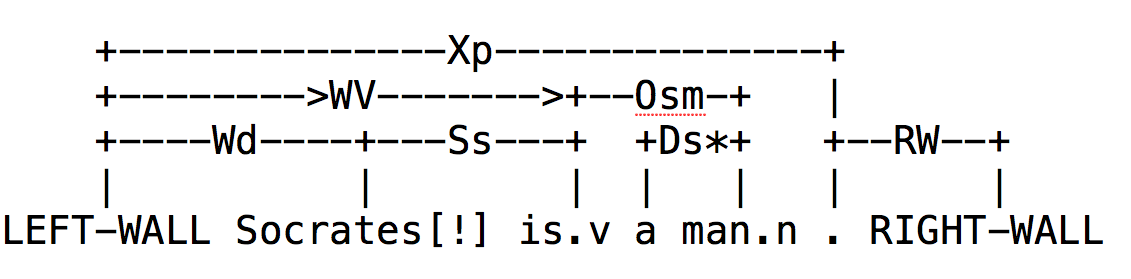
\includegraphics[width=12cm]{Socrates_1.png}

\begin{verbatim}
Dependency relations:

    _obj(be, man)
    _subj(be, Socrates)

Attributes:

    tense(be, present)
    subscript-TAG(be, .v)
    pos(be, verb)
    pos(., punctuation)
    subscript-TAG(man, .n)
    pos(man, noun)
    noun_number(man, singular)
    definite-FLAG(Socrates, T)
    pos(Socrates, noun)
    noun_number(Socrates, singular)
    pos(a, det)

\end{verbatim}


\begin{verbatim}
((ReferenceLink
   (InterpretationNode "sentence@f04de205-0f67-471d-84fc-2f9c6103ebca_parse_0_interpretation_$X")
   (SetLink
      (InheritanceLink
         (ConceptNode "Socrates@cfbb87d6-5444-4845-a673-8d70b93ffde6")
         (ConceptNode "Socrates" (ptv 1 0 1))
      )
      (InheritanceLink
         (ConceptNode "man@fe411437-7607-4169-abcf-d42ebcd50338")
         (ConceptNode "man" (ptv 1 0 1))
      )
      (InheritanceLink
         (ConceptNode "Socrates@cfbb87d6-5444-4845-a673-8d70b93ffde6")
         (ConceptNode "man@fe411437-7607-4169-abcf-d42ebcd50338")
      )
      (ImplicationLink
         (PredicateNode "is@b06a386e-0983-4bc8-bd1e-395b487faff2")
         (PredicateNode "be" (ptv 1 0 1))
      )
      (InheritanceLink
         (PredicateNode "is@b06a386e-0983-4bc8-bd1e-395b487faff2")
         (ConceptNode "present")
      )
      (InheritanceLink
         (InterpretationNode "sentence@f04de205-0f67-471d-84fc-2f9c6103ebca_parse_0_interpretation_$X")
         (ConceptNode "DeclarativeSpeechAct")
      )
      (EvaluationLink
         (PredicateNode "definite")
         (ListLink
            (ConceptNode "Socrates@cfbb87d6-5444-4845-a673-8d70b93ffde6")
         )
      )
   )
)
)
\end{verbatim}

\noindent {\bf Example 2: } Men breathe air.

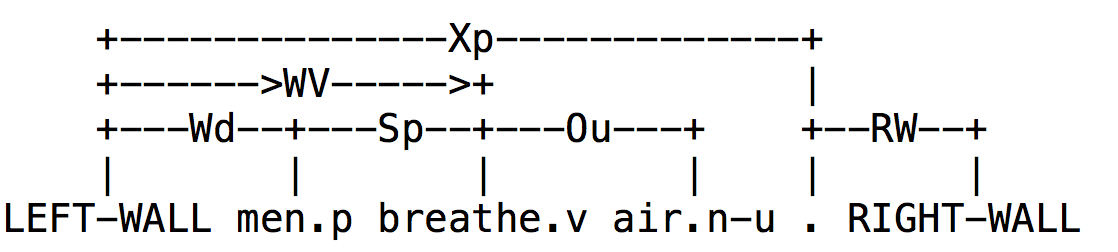
\includegraphics[width=12cm]{Socrates_2.png}

\begin{verbatim}

Dependency relations:

    _obj(breathe, air)
    _subj(breathe, man)

Attributes:

    tense(breathe, present)
    subscript-TAG(breathe, .v)
    pos(breathe, verb)
    pos(., punctuation)
    subscript-TAG(air, .n-u)
    pos(air, noun)
    noun_number(air, uncountable)
    subscript-TAG(man, .p)
    pos(man, noun)
    noun_number(man, plural)

\end{verbatim}

\begin{verbatim}
((ReferenceLink
   (InterpretationNode "sentence@05b9ba83-e424-43c8-b5f1-8261217bc548_parse_0_interpretation_$X")
   (SetLink
      (ImplicationLink
         (PredicateNode "breathe@ba9dec0b-b99f-4c2c-a5cc-31cc9aa4f172")
         (PredicateNode "breathe" (ptv 1 0 1))
      )
      (InheritanceLink
         (ConceptNode "men@5f6e723d-e57e-47e5-89df-ee9daaa2936d")
         (ConceptNode "man" (ptv 1 0 2))
      )
      (InheritanceLink
         (ConceptNode "air@98afd45c-4807-4607-a732-298c7979327f")
         (ConceptNode "air" (ptv 1 0 1))
      )
      (EvaluationLink
         (PredicateNode "breathe@ba9dec0b-b99f-4c2c-a5cc-31cc9aa4f172")
         (ListLink
            (ConceptNode "men@5f6e723d-e57e-47e5-89df-ee9daaa2936d")
            (ConceptNode "air@98afd45c-4807-4607-a732-298c7979327f")
         )
      )
      (InheritanceLink
         (PredicateNode "breathe@ba9dec0b-b99f-4c2c-a5cc-31cc9aa4f172")
         (ConceptNode "present")
      )
      (InheritanceLink
         (InterpretationNode "sentence@05b9ba83-e424-43c8-b5f1-8261217bc548_parse_0_interpretation_$X")
         (ConceptNode "DeclarativeSpeechAct")
      )
   )
)
)
\end{verbatim}


\noindent {\bf Example 3: }  Socrates breathes air.

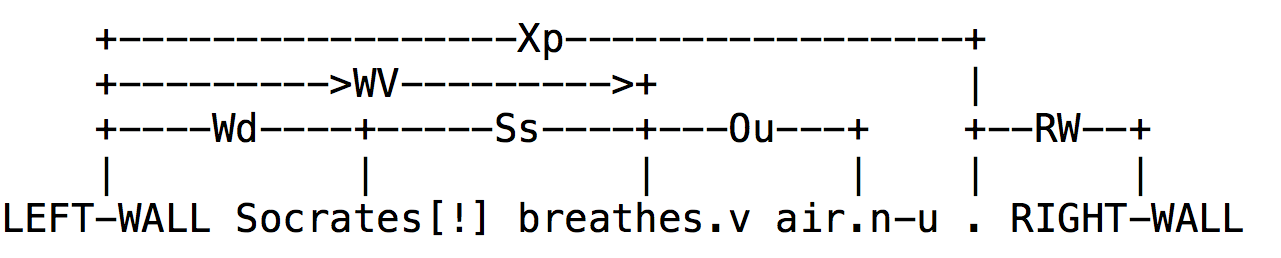
\includegraphics[width=12cm]{Socrates_3.png}

\begin{verbatim}

Dependency relations:

    _obj(breathe, air)
    _subj(breathe, Socrates)

Attributes:

    tense(breathe, present)
    subscript-TAG(breathe, .v)
    pos(breathe, verb)
    pos(., punctuation)
    subscript-TAG(air, .n-u)
    pos(air, noun)
    noun_number(air, uncountable)
    definite-FLAG(Socrates, T)
    pos(Socrates, noun)
    noun_number(Socrates, singular)

\end{verbatim}


\begin{verbatim}
((ReferenceLink
   (InterpretationNode "sentence@a41e5f83-4a87-4c3f-ad39-833510272d90_parse_0_interpretation_$X")
   (SetLink
      (ImplicationLink
         (PredicateNode "breathes@0a04573a-c867-458d-baa9-0f347ee73371")
         (PredicateNode "breathe" (ptv 1 0 2))
      )
      (InheritanceLink
         (ConceptNode "Socrates@a34bbdf7-1dac-4e62-9dfa-48e1a1f9710c")
         (ConceptNode "Socrates" (ptv 1 0 2))
      )
      (InheritanceLink
         (ConceptNode "air@016cb5c7-35b7-42c4-8690-e3958030773f")
         (ConceptNode "air" (ptv 1 0 2))
      )
      (EvaluationLink
         (PredicateNode "breathes@0a04573a-c867-458d-baa9-0f347ee73371")
         (ListLink
            (ConceptNode "Socrates@a34bbdf7-1dac-4e62-9dfa-48e1a1f9710c")
            (ConceptNode "air@016cb5c7-35b7-42c4-8690-e3958030773f")
         )
      )
      (InheritanceLink
         (PredicateNode "breathes@0a04573a-c867-458d-baa9-0f347ee73371")
         (ConceptNode "present")
      )
      (InheritanceLink
         (InterpretationNode "sentence@a41e5f83-4a87-4c3f-ad39-833510272d90_parse_0_interpretation_$X")
         (ConceptNode "DeclarativeSpeechAct")
      )
      (EvaluationLink
         (PredicateNode "definite")
         (ListLink
            (ConceptNode "Socrates@a34bbdf7-1dac-4e62-9dfa-48e1a1f9710c")
         )
      )
   )
)
)
\end{verbatim}


\noindent {\bf Example 4: }  I think Socrates is a man.

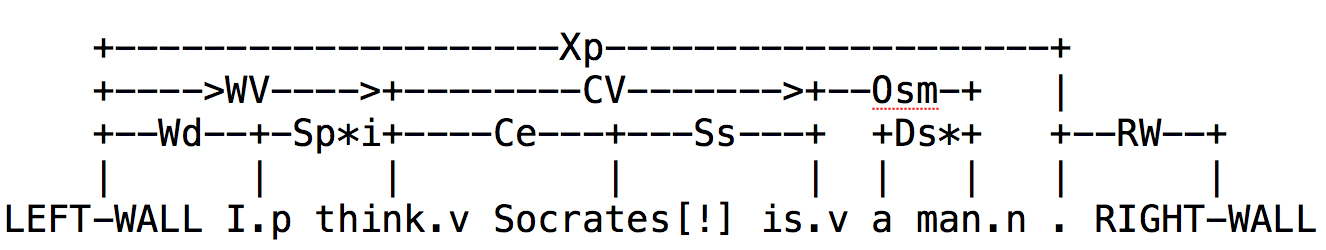
\includegraphics[width=12cm]{Socrates_4.png}

\begin{verbatim}

Dependency relations:

    _obj(be, man)
    _subj(be, Socrates)
    _rep(think, be)
    _subj(think, I)

Attributes:

    definite-FLAG(Socrates, T)
    pos(Socrates, noun)
    noun_number(Socrates, singular)
    pos(., punctuation)
    subscript-TAG(man, .n)
    pos(man, noun)
    noun_number(man, singular)
    pos(a, det)
    tense(be, present)
    HYP(be, T)
    subscript-TAG(be, .v)
    pos(be, verb)
    tense(think, present)
    subscript-TAG(think, .v)
    pos(think, verb)
    pronoun-FLAG(I, T)
    gender(I, person)
    definite-FLAG(I, T)
    subscript-TAG(I, .p)
    pos(I, noun)
    noun_number(I, singular)

\end{verbatim}


\begin{verbatim}

((ReferenceLink
   (InterpretationNode "sentence@ec1ca4d5-20ce-465c-9686-aa3edd4dbb2f_parse_0_interpretation_$X")
   (SetLink
      (ImplicationLink
         (PredicateNode "think@8be218e8-095b-44e7-b321-ee877fe4ad45")
         (PredicateNode "think" (ptv 1 0 1))
      )
      (InheritanceLink
         (ConceptNode "I@8c841336-dc92-4c3a-a5af-2e860365ff88")
         (ConceptNode "I" (ptv 1 0 1))
      )
      (EvaluationLink
         (PredicateNode "think@8be218e8-095b-44e7-b321-ee877fe4ad45")
         (ListLink
            (ConceptNode "I@8c841336-dc92-4c3a-a5af-2e860365ff88")
         )
      )
      (ImplicationLink
         (PredicateNode "is@14df1d2f-f71e-45c9-b4a3-80eb38c6a89f")
         (PredicateNode "be" (ptv 1 0 2))
      )
      (EvaluationLink
         (PredicateNode "think@8be218e8-095b-44e7-b321-ee877fe4ad45")
         (ListLink
            (ConceptNode "is@14df1d2f-f71e-45c9-b4a3-80eb38c6a89f")
         )
      )
      (InheritanceLink
         (PredicateNode "think@8be218e8-095b-44e7-b321-ee877fe4ad45")
         (ConceptNode "present")
      )
      (InheritanceLink
         (ConceptNode "Socrates@c1fde686-ae83-45e8-a60d-259179597e68")
         (ConceptNode "Socrates" (ptv 1 0 3))
      )
      (EvaluationLink
         (PredicateNode "definite")
         (ListLink
            (ConceptNode "Socrates@c1fde686-ae83-45e8-a60d-259179597e68")
         )
      )
      (InheritanceLink
         (InterpretationNode "sentence@ec1ca4d5-20ce-465c-9686-aa3edd4dbb2f_parse_0_interpretation_$X")
         (ConceptNode "DeclarativeSpeechAct")
      )
      (InheritanceLink
         (ConceptNode "man@aed74351-8482-4a5b-a6f4-3e979b537fae")
         (ConceptNode "man" (ptv 1 0 3))
      )
      (InheritanceLink
         (ConceptNode "Socrates@c1fde686-ae83-45e8-a60d-259179597e68")
         (ConceptNode "man@aed74351-8482-4a5b-a6f4-3e979b537fae")
      )
      (InheritanceLink
         (PredicateNode "is@14df1d2f-f71e-45c9-b4a3-80eb38c6a89f")
         (ConceptNode "present")
      )
      (EvaluationLink
         (PredicateNode "definite")
         (ListLink
            (ConceptNode "I@8c841336-dc92-4c3a-a5af-2e860365ff88")
         )
      )
   )
)
)
\end{verbatim}


\noindent {\bf Example 5: }  Bob thinks Socrates is a woman.

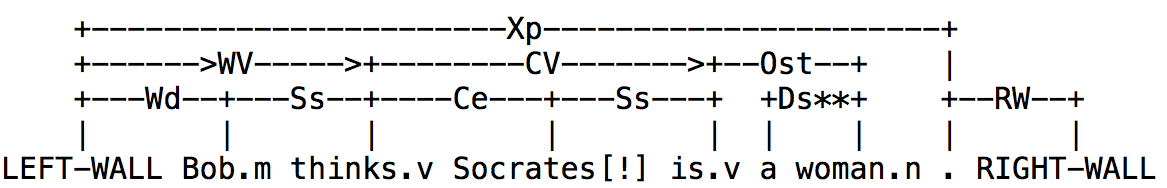
\includegraphics[width=12cm]{Socrates_5.png}

\begin{verbatim}

Dependency relations:

    _obj(be, woman)
    _subj(be, Socrates)
    _rep(think, be)
    _subj(think, Bob)

Attributes:

    definite-FLAG(Socrates, T)
    pos(Socrates, noun)
    noun_number(Socrates, singular)
    pos(., punctuation)
    subscript-TAG(woman, .n)
    pos(woman, noun)
    noun_number(woman, singular)
    pos(a, det)
    tense(be, present)
    HYP(be, T)
    subscript-TAG(be, .v)
    pos(be, verb)
    tense(think, present)
    subscript-TAG(think, .v)
    pos(think, verb)
    gender(Bob, masculine)
    definite-FLAG(Bob, T)
    person-FLAG(Bob, T)
    subscript-TAG(Bob, .m)
    pos(Bob, noun)
    noun_number(Bob, singular)

\end{verbatim}


\begin{verbatim}

((ReferenceLink
   (InterpretationNode "sentence@8c6d9ca7-abc8-4dbd-8442-669e62a32cc0_parse_0_interpretation_$X")
   (SetLink
      (ImplicationLink
         (PredicateNode "thinks@87f3ac28-56e7-44fc-8125-815b2e6747ee")
         (PredicateNode "think" (ptv 1 0 2))
      )
      (InheritanceLink
         (ConceptNode "Bob@f16c5987-7193-4809-9a3f-94c73a77d4d4")
         (ConceptNode "Bob" (ptv 1 0 1))
      )
      (EvaluationLink
         (PredicateNode "thinks@87f3ac28-56e7-44fc-8125-815b2e6747ee")
         (ListLink
            (ConceptNode "Bob@f16c5987-7193-4809-9a3f-94c73a77d4d4")
         )
      )
      (ImplicationLink
         (PredicateNode "is@712b5da0-e4df-4b24-9bca-e0a1114a6854")
         (PredicateNode "be" (ptv 1 0 3))
      )
      (EvaluationLink
         (PredicateNode "thinks@87f3ac28-56e7-44fc-8125-815b2e6747ee")
         (ListLink
            (ConceptNode "is@712b5da0-e4df-4b24-9bca-e0a1114a6854")
         )
      )
      (InheritanceLink
         (PredicateNode "thinks@87f3ac28-56e7-44fc-8125-815b2e6747ee")
         (ConceptNode "present")
      )
      (InheritanceLink
         (ConceptNode "Socrates@eadf1215-ca8d-42ee-88b9-ac1e6471f8c1")
         (ConceptNode "Socrates" (ptv 1 0 4))
      )
      (EvaluationLink
         (PredicateNode "definite")
         (ListLink
            (ConceptNode "Socrates@eadf1215-ca8d-42ee-88b9-ac1e6471f8c1")
         )
      )
      (InheritanceLink
         (InterpretationNode "sentence@8c6d9ca7-abc8-4dbd-8442-669e62a32cc0_parse_0_interpretation_$X")
         (ConceptNode "DeclarativeSpeechAct")
      )
      (InheritanceLink
         (ConceptNode "woman@9d719ddc-0fe5-4171-a4e5-5397a6c6e9e9")
         (ConceptNode "woman" (ptv 1 0 1))
      )
      (InheritanceLink
         (ConceptNode "Socrates@eadf1215-ca8d-42ee-88b9-ac1e6471f8c1")
         (ConceptNode "woman@9d719ddc-0fe5-4171-a4e5-5397a6c6e9e9")
      )
      (InheritanceLink
         (PredicateNode "is@712b5da0-e4df-4b24-9bca-e0a1114a6854")
         (ConceptNode "present")
      )
      (InheritanceLink
         (SpecificEntityNode "Bob@f16c5987-7193-4809-9a3f-94c73a77d4d4")
         (ConceptNode "male")
      )
      (InheritanceLink
         (SpecificEntityNode "Bob@f16c5987-7193-4809-9a3f-94c73a77d4d4")
         (ConceptNode "Bob" (ptv 1 0 1))
      )
      (EvaluationLink
         (PredicateNode "definite")
         (ListLink
            (ConceptNode "Bob@f16c5987-7193-4809-9a3f-94c73a77d4d4")
         )
      )
   )
)
)

\end{verbatim}


%%%%%%%%%%%%%%%%%%%%%%%%%%%%%%%%%%%%%%%%%%%%%%%%%%%%%%%%%%%%%%%
\section{本章小结}{Summary of Accomplishments and Future Work}
%%%%%%%%%%%%%%%%%%%%%%%%%%%%%%%%%%%%%%%%%%%%%%%%%%%%%%%%%%%%%%%

本章主要介绍我们的自然语言理解系统中的各个模块的工作原理和实现方法,并深入讨论了该系统如何将英文句子转换成超图表示的逻辑形式,以达到能使自然语言参与到逻辑推理的过程中。该自然语言理解系统已经被应用在游戏角色控制和人形机器人等领域。

该自然语言理解系统使用了一些现有的开源语法分析器,本章也讨论对这些开源工具做出的各种改进,还讨论了我们实现的全新的将依存关系转换成语义逻辑表示的系统RelEx2Logic,总的来说,本章的贡献有:

\begin{itemize}
\item 改进了链语法分析器的词典,使其能够处理更复杂的语言现象,以及能识别句子的中心词从而改进了链语法对复句的分析能力。
\item 改进了RelEx使其能处理目前语法分析器难以处理的比较级和量词等复杂的语言现象。
\item 设计并实现了RelEx2Logic系统,使其能将RelEx输出的依存关系转换成以超图表示的逻辑形式
\item 设计并实现了RelEx2Logic中所使用的转换规则及相应的规则引擎。
\end{itemize}

总的来说,本章搭建的自然语言理解系统已经能被用在一些用户定义的实际应用中,但仍然有很多遗留问题有待解决。在接下来的工作中,我们会在我们的自然语言理解系统中引入概率逻辑推理引擎PLN,这样不仅可以通过一些基本常识推理来改进语法分析中的结果,还可用于指导对语法分析器产生的多种结果进行排序,以及用于指导各种歧义消除和指代消解等方面。除此之外,我们还致力通过无监督的机器学习方法从大型文本语料学习相关的语法规则,来替代当前系统中使用的人工编写的规则库,本文会在第\ref{chap:learning}章中对此做更深入的讨论。


参考文献:
1 “Parsing with a Link Grammar”
2 G. Schneider, ``Learning to Disambiguate Syntactic
Relations''
3 frequent subtree mining
4 word grammar
